\section{Testing Strategy and Objectives}
\label{sec:testing_strategy}

Chapter~\ref{chap:system_implementation} described how the control-plane backend orchestrates tenant databases on Kubernetes through CloudNativePG, the MongoDB Community Operator, PGProxy, and a REST API written in Go. This chapter is the verification counterpart to that implementation: it documents the automated test suite that validates the backend's business logic, and the code-coverage methodology used to measure and improve how much of that logic is exercised.

The chapter is deliberately titled \emph{Unit and Component Testing} rather than \emph{system testing}. In the standard software-engineering taxonomy, system testing exercises the fully integrated product against its requirements; what this chapter documents is the layer beneath that: automated tests of the control-plane backend's Go packages, in which every external dependency is replaced by an in-process double. The suite verifies the Go binary that exposes the REST API, performs request validation, maps domain errors to HTTP responses, executes SQL against tenant databases, manages MongoDB collections, and handles authentication. It does not drive a live Kubernetes cluster or real database engines; that boundary is deliberate and is justified below. Figure~\ref{fig:testing_pyramid} positions this work within the classical testing pyramid: it occupies the broad unit/component base, while integration and end-to-end testing on a live \texttt{k3d} cluster are identified as complementary future work (Section~\ref{sec:testing_limitations}).

\begin{figure}[H]
    \centering
    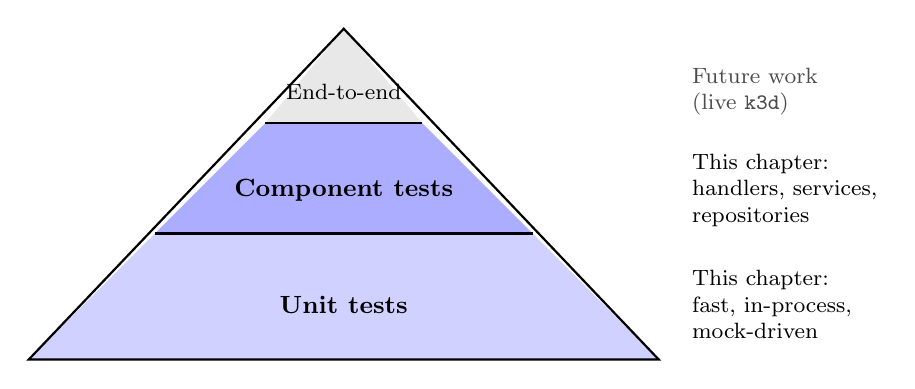
\begin{tikzpicture}[scale=1.0, every node/.style={font=\small}]
        % Pyramid layers (bottom = widest)
        \fill[blue!18]   (-4,0) -- (4,0) -- (2.4,1.6) -- (-2.4,1.6) -- cycle;
        \fill[blue!32]   (-2.4,1.6) -- (2.4,1.6) -- (1.0,3.0) -- (-1.0,3.0) -- cycle;
        \fill[gray!18]   (-1.0,3.0) -- (1.0,3.0) -- (0,4.2) -- cycle;
        % Outline
        \draw[thick] (-4,0) -- (4,0) -- (0,4.2) -- cycle;
        \draw[thick] (-2.4,1.6) -- (2.4,1.6);
        \draw[thick] (-1.0,3.0) -- (1.0,3.0);
        % Labels inside
        \node at (0,0.7)  {\textbf{Unit tests}};
        \node at (0,2.15) {\textbf{Component tests}};
        \node[font=\footnotesize] at (0,3.4) {End-to-end};
        % Side annotations
        \node[right, align=left, font=\footnotesize] at (4.3,0.7)
            {This chapter:\\fast, in-process,\\mock-driven};
        \node[right, align=left, font=\footnotesize] at (4.3,2.15)
            {This chapter:\\handlers, services,\\repositories};
        \node[right, align=left, font=\footnotesize, text=gray!60!black] at (4.3,3.4)
            {Future work\\(live \texttt{k3d})};
    \end{tikzpicture}
    \caption{The testing pyramid. This chapter's suite occupies the unit and component layers; end-to-end testing on a live cluster is treated as future work (Section~\ref{sec:testing_limitations}).}
    \label{fig:testing_pyramid}
\end{figure}

\subsection{Scope and Goals}

The test suite was written to satisfy the following objectives:

\begin{itemize}
    \item \textbf{Correctness of business logic.} Confirm that service-layer operations --- project creation, table DDL generation, row manipulation, collection management, and authentication --- produce the expected results for valid inputs.
    \item \textbf{Validation rules.} Verify that the backend rejects malformed or unsafe input before it reaches a tenant database: invalid database types, weak passwords, unknown resource tiers, illegal identifiers, and multi-statement SQL.
    \item \textbf{Error-path behavior.} Exercise negative paths so that downstream failures (a missing project, a duplicate resource, an unreachable upstream service, a cancelled request) are mapped to the correct error identity and HTTP status code rather than surfacing as unhandled panics.
    \item \textbf{Regression safety.} Provide a fast, deterministic suite that can be run on every change (\texttt{go test ./...}) so that refactoring the backend does not silently break existing behavior.
\end{itemize}

\subsection{Why a Deterministic, Mock-Driven Approach}

The backend's natural dependencies --- PostgreSQL, MongoDB, Redis, the Kubernetes API, and the external Schema-AI service --- are precisely the components that make end-to-end tests slow, environment-sensitive, and flaky; standing up a real cluster per run would couple correctness checks to provisioning latency (20--31 seconds per project, Section~\ref{sec:performance_evaluation}) and to network availability. The suite therefore runs entirely in process, with no live services and no network: every such dependency is replaced by an in-memory fake, a mock, or a local test server. This keeps the full suite running in seconds, makes failures reproducible, and lets it run unchanged in continuous integration where no cluster exists. Testing against a live \texttt{k3d} cluster is treated as complementary future work (Section~\ref{sec:testing_limitations}), not a substitute for this fast inner loop.

\subsection{Test Automation and Execution}
\label{sec:test_automation}

The suite is not a one-off exercise; it is wired into the development workflow. In total it comprises roughly \textbf{676 test functions across 18 packages}, making on the order of 1{,}700 assertions, all invoked with the single command \texttt{go test ./...}, which compiles and runs every package's tests in parallel. On a developer laptop the complete suite --- compilation included --- finishes in approximately \textbf{22 seconds} of wall-clock time, fast enough to run before every commit without disrupting the inner development loop.

Because every dependency is an in-process double, the suite is fully deterministic: no test is skipped or marked as known-failing, and repeated executions --- locally and in CI, with the test cache disabled via \texttt{-count=1} --- produce identical results with no flaky failures. This is a direct consequence of the no-network design rather than an accident of timing.

The same command runs automatically in continuous integration. A GitHub Actions workflow triggers on every pull request: it checks out the repository, provisions the pinned Go toolchain, builds the entire module with \texttt{go build ./...}, and then executes \texttt{go test ./...}. Because the suite has no external dependencies, the CI runner needs no database, cluster, or network services --- the same property that makes the tests deterministic locally makes them portable to a clean CI environment. A failing test fails the workflow, surfacing regressions at review time before a change is merged.
